\section{自由链复形的上同调}
\sourcepage{331}
到目前为止只计算了少数简单空间的上同调。第 5.8 节将证明：CW 复形的胞腔链复形不但计算同调，也计算上同调。证明依赖本节关于自由链复形的两个定理。

第一个定理说，同调群间任意一族同态都由某个链映射诱导；第二个说，自由链复形间诱导同调同构的链映射也诱导上同调同构。第七章还会独立证明第二个定理，读者也可暂时接受它。

\sourcepage{332}
\entry{定义}{5.6.1}若短正合列 $0\to A\to B\to C\to0$ 中 $A,B$ 自由，则称为 $C$ 的\textbf{自由消解}（free resolution）。任意阿贝尔群都有自由消解：取以 $C$ 的元素为生成元的自由阿贝尔群 $B$，令 $A$ 为自然投影的核。这称为\textbf{典范自由消解}（canonical free resolution）。

自由消解有如下提升性质：给定两条短正合列及 $\gamma:C\to C'$，若第一列的 $A,B$ 自由，则存在 $\beta:B\to B'$、$\alpha:A\to A'$，使整个图交换。证明是：选 $B$ 的基，对每个基元 $b$，在满射 $\psi':B'\to C'$ 下选择 $\gamma\psi(b)$ 的一个原像作为 $\beta(b)$，再线性延拓。它将 $\operatorname{im}\varphi$ 映到 $\operatorname{im}\varphi'$，由后者的单射性确定 $\alpha$。\translatornote{原书选择原像的表达式中把基元 $b$ 误写为整个群 $B$。}

\entry{定理}{5.6.2}若 $\mathcal C,\mathcal C'$ 自由，给定所有维数的同态 $\gamma:H_p(\mathcal C)\to H_p(\mathcal C')$，则存在诱导它们的链映射 $\varphi$。更强地，任何诱导 $\gamma$ 的闭链群同态族 $\beta:Z_p\to Z'_p$ 都可延拓为链映射。

\textbf{证明：}边缘群与闭链群均为自由阿贝尔群。对短正合列 $0\to B_p\to Z_p\to H_p\to0$ 应用上述提升性质，得相容的 $\alpha:B_p\to B'_p$、$\beta:Z_p\to Z'_p$。若 $\beta$ 已给定，$\alpha$ 就取其在边缘群上的限制。

\sourcepage{333}
短正合列 $0\to Z_p\to C_p\to B_{p-1}\to0$ 分裂，故可选
\[
C_p=Z_p\oplus U_p,\qquad C'_p=Z'_p\oplus U'_p,
\]
边缘在 $U_p,U'_p$ 上分别给出到 $B_{p-1},B'_{p-1}$ 的同构。定义 $\varphi$ 在 $Z_p$ 上为 $\beta$，在 $U_p$ 上为经这些同构由 $\alpha$ 诱导的映射。因此 $\partial'\varphi=\alpha\partial$，而在低一维边缘群上 $\varphi=\beta=\alpha$。于是 $\partial'\varphi=\varphi\partial$，它是链映射。闭链上的限制为 $\beta$，所以诱导的同调同态正是 $\gamma$。\hfill$\square$

\entry{推论}{5.6.3}对自由增广链复形，任意约化同调同态族都由保持增广的链映射诱导。

\textbf{证明：}把增广群 $\Z$ 放在负一维，增广作为边缘。负一维同调为零，在该维选闭链映射为恒等，其余维选诱导所给同调同态的闭链映射，应用上一定理。所得链映射自动保持增广。\hfill$\square$

\sourcepage{334}
\entry{引理}{5.6.4}若自由链复形短正合列 $0\to\mathcal C\xrightarrow{\varphi}\mathcal D\to\mathcal E\to0$ 中 $\varphi$ 在所有维数诱导同调同构，则也诱导上同调同构。

\textbf{证明：}同调长正合列说明 $H_p(\mathcal E)=0$。记 $\mathcal E$ 的边缘、闭链为 $B_p,Z_p$。因自由性，$E_p=Z_p\oplus U_p=B_p\oplus U_p$，且边缘将 $U_p$ 同构地映到 $B_{p-1}$、在 $B_p$ 上为零。对偶后
\[
\operatorname{Hom}(E_p,G)\cong\operatorname{Hom}(B_p,G)\oplus\operatorname{Hom}(U_p,G),
\]
上边缘将第一项同构地映到下一维的 $\operatorname{Hom}(U_{p+1},G)$，并在第二项上为零。因此上闭链恰为上一维的上边缘，$H^p(\mathcal E;G)=0$。原短正合列逐维分裂，上同调长正合列遂给出结论。\hfill$\square$

上一节实际只用到这个特殊情形。一般情形借助下面的引理归结于它。

\entry{引理}{5.6.5}给定自由链复形间的链映射 $\varphi:\mathcal C\to\mathcal D$，存在自由链复形 $\mathcal D'$ 及单射链映射 $i:\mathcal C\to\mathcal D'$、$j:\mathcal D\to\mathcal D'$，使 $i$ 链同伦于 $j\varphi$，$j$ 诱导所有维数的同调同构，且两个商复形均自由。

\textbf{证明：}这一看似凭空引入的构造称为 $\varphi$ 的\textbf{代数映射柱}（algebraic mapping cylinder），后面说明其几何动机。令
\[
D'_p=C_p\oplus D_p\oplus C_{p-1},\qquad
\partial'(c,d,b)=(\partial c-b,\partial d+\varphi b,-\partial b).
\]
容易验证 $\partial'^2=0$，两个自然包含是链映射，链群及商群都自由。令 $D(c)=(0,0,c)$，则 $\partial'D+D\partial=j\varphi-i$。

\sourcepage{335}
为证 $j$ 诱导同构，只需说明商 $\mathcal D'/\mathcal D$ 同调为零。其链群为 $C_p\oplus C_{p-1}$，边缘为 $\partial''(c,b)=(\partial c-b,-\partial b)$。若 $(c,b)$ 闭，则 $b=\partial c$，从而 $(c,b)=(c,\partial c)=-\partial''(0,c)$，故每个闭链都为边缘。\hfill$\square$

\entry{定理}{5.6.6}自由链复形间的链映射若在每一维诱导同调同构，则在每一维、对任意系数群也诱导上同调同构。

\textbf{证明：}取上一个引理的 $i,j$。因 $j,\varphi$ 都诱导同调同构，而 $i\simeq j\varphi$，$i$ 也如此。对自由商短正合列分别应用引理 5.6.4，得 $i^*,j^*$ 都为同构。又 $i^*=\varphi^*j^*$，故 $\varphi^*$ 为同构。\hfill$\square$

\sourcepage{336}
\entry{推论}{5.6.7}若两个自由链复形在所有维数的同调群同构，则它们在所有维数、任意系数群的上同调群也同构。

\entry{注}{5.6.8}解释映射柱的几何动机。给定 $h:X\to Y$，可构造空间 $Y'$ 及嵌入 $i:X\to Y'$、$j:Y\to Y'$，使 $i\simeq jh$，且 $j$ 为同伦等价。这样 $h$ 为同伦等价当且仅当 $i$ 为同伦等价，把任意映射的问题化为嵌入的问题。

具体地，在拓扑和 $(X\times I)\amalg Y$ 中，把 $(x,0)$ 与 $h(x)$ 认同，所得粘合空间称为 $h$ 的\textbf{映射柱}（mapping cylinder），形似高顶礼帽。$j$ 为 $Y$ 的包含，$i(x)=\pi(x,1)$。把礼帽压到底面，就得到 $Y'$ 到 $j(Y)$ 的形变收缩，也得到 $i$ 与 $jh$ 的同伦。
\begin{center}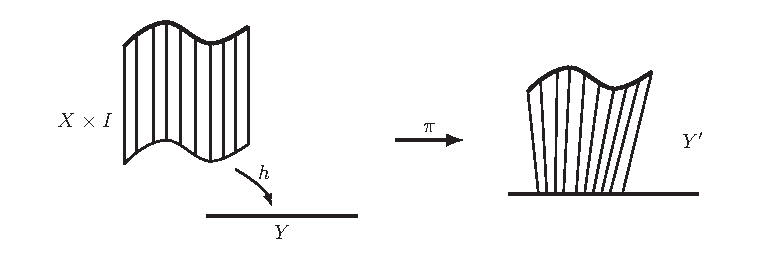
\includegraphics[width=.96\textwidth]{figures/5-6-1.pdf}\\图 5.6.1\end{center}

\sourcepage{337}
若作适当三角剖分，使 $i(X),j(Y)$ 及每个柱 $\pi(\sigma\times I)$ 都为子复形，可把柱分成三类开 $p$ 维胞腔：顶面的 $p$ 维开单形、底面的 $p$ 维开单形，以及中间的 $(p-1)$ 维单形乘开区间。因此胞腔链群正是
\[
C_p(X)\oplus C_p(Y)\oplus C_{p-1}(X).
\]
前两项上边缘分别是原来的边缘。第三类胞腔的边缘由柱的上下两面及侧面组成。粘合后，它具有 $h_\#\sigma-\sigma\pm(\partial\sigma)\times I$ 的形式，写成三元组就是 $(-\sigma,h_\#\sigma,\pm\partial\sigma)$。为使边缘平方为零，末项必须取负号，这恰是代数映射柱的定义。

下面给出一个联系同调与上同调的应用，第七章将推广它。

\entry{定义}{5.6.9}双线性\textbf{取值映射} $\operatorname{Hom}(C_p,G)\times C_p\to G$ 诱导配对
\[
H^p(\mathcal C;G)\times H_p(\mathcal C)\to G,
\]
称为\textbf{Kronecker 指标}（Kronecker index），仍记为 $\langle\alpha^p,\beta_p\rangle$。

\sourcepage{338}
\entry{引理}{5.6.10}Kronecker 指标良定义。

\textbf{证明：}若 $z_p$ 闭、$z^p$ 上闭，则改变代表后的取值为
\begin{align*}
\langle z^p+\delta d^{p-1},z_p+\partial d_{p+1}\rangle
&=\langle z^p,z_p\rangle+\langle d^{p-1},\partial z_p\rangle\\
&\quad+\langle\delta z^p,d_{p+1}\rangle+\langle d^{p-1},\partial^2d_{p+1}\rangle
=\langle z^p,z_p\rangle.
\end{align*}
\hfill$\square$

\entry{定义}{5.6.11}\textbf{Kronecker 映射}
\[
\kappa:H^p(\mathcal C;G)\to\operatorname{Hom}(H_p(\mathcal C),G)
\]
定义为 $(\kappa\alpha)(\beta)=\langle\alpha,\beta\rangle$。由第一变量线性性，它是同态；自然性留作习题 2。

\entry{引理}{5.6.12}若 $\mathcal C$ 自由，则存在自然短正合列
\[
0\leftarrow\operatorname{Hom}(H_p(\mathcal C),G)\xleftarrow{\kappa}H^p(\mathcal C;G)
\leftarrow\ker\kappa\leftarrow0.
\]
它分裂，但分裂不自然。本引理不依赖本节前面的定理。

\textbf{证明：}构造 $\lambda^*$ 使 $\kappa\lambda^*$ 为恒等。由于 $Z_p$ 是 $C_p$ 的直和项，投影 $\pi:Z_p\to H_p(\mathcal C)$ 可延拓为 $\lambda:C_p\to H_p(\mathcal C)$。令 $E_p=H_p(\mathcal C)$，所有边缘为零，则 $H_p(\mathcal E)=E_p$，$H^p(\mathcal E;G)=\operatorname{Hom}(H_p(\mathcal C),G)$。因为 $\lambda$ 在边缘上为零，它是链映射，且在同调上诱导恒等。

\sourcepage{339}
其上同调映射未必为同构，但对任意 $\gamma:H_p(\mathcal C)\to G$ 及闭链 $z_p$，有
\[
(\kappa\lambda^*\gamma)(\{z_p\})=\langle\gamma,\lambda(z_p)\rangle=\gamma(\{z_p\}).
\]
因此复合为恒等，证明分裂与满射性。\hfill$\square$

\entry{定理}{5.6.13}若自由链复形的所有同调群也自由，则 $\kappa$ 在所有维数均为同构。

\textbf{证明：}上一证明中的 $\mathcal E$ 此时自由，且 $\lambda$ 诱导同调同构。由定理 5.6.6，$\lambda^*$ 为同构。因 $\kappa\lambda^*$ 为恒等，$\kappa$ 也是同构。\hfill$\square$

因此，自由同调情形下，上同调自然等于同调的对偶群。第七章将推广这一结论；实际上只需单个 $H_{p-1}(\mathcal C)$ 自由即可。

\subsection*{习题}
\begin{enumerate}
\item 验证引理 5.6.5 的边缘平方为零。
\item \begin{enumerate}[label=(\alph*)]
\item 证明对链映射 $\varphi:\mathcal C\to\mathcal D$，有 $\kappa_{\mathcal C}\varphi^*=\overline{\varphi_*}\kappa_{\mathcal D}$，即 Kronecker 映射自然。
\item 配对在两个变量上变性相反，直接表述自然性较不便。证明 $\langle\varphi^*\alpha,\beta\rangle=\langle\alpha,\varphi_*\beta\rangle$。
\end{enumerate}
\item 设 $H_n(X),H^n(X),H_n(Y),H^n(Y)$ 都为无限循环群，$f:X\to Y$ 连续。若 $f_*$ 为乘以 $d$，证明除符号选择外，$f^*$ 也为乘以 $d$。〔提示：证明 $\kappa$ 为同构。〕
\item 引理 5.6.12 的延拓 $\lambda$ 涉及任意选择，证明分裂确实不自然。
\begin{enumerate}[label=(\alph*)]
\item 找自由链复形及链映射 $\varphi:\mathcal C\to\mathcal D$，使无论怎样选择，两条分裂 $\lambda^*$ 都不能满足 $\varphi^*\lambda_{\mathcal D}^*=\lambda_{\mathcal C}^*\overline{\varphi_*}$。
\item 〔*〕找空间及连续映射，使其奇异链复形实现 (a) 的情形。
\end{enumerate}
\item 求 $\Z/n$ 的一个自由消解。
\end{enumerate}
